\documentclass[preprint, hmargin=1in, vmargin=1in]{aastex62}
%%%%%%begin preamble
%\usepackage[hmargin=1in, vmargin=1in]{geometry} % Margins
\usepackage{hyperref}
\usepackage{url}
\usepackage{natbib}
\setlength{\bibsep}{0pt plus 0.3ex}
\usepackage{graphicx}
\usepackage{amsmath}
\usepackage{amsfonts}
\usepackage{amssymb}
%\usepackage{import}
\usepackage{wrapfig}


\usepackage{color}
\hypersetup{
  colorlinks   = true,
  %citecolor    = blue
  citecolor    = gray
  % gray is not being found!?!
  % gray is found if pdfpages is used... crap.
  %citecolor    = grey
  %citecolor    = Gray
}

%% headers
\usepackage{fancyhdr}
\pagestyle{fancy}
\fancyhf{} % sets both header and footer to nothing
\lhead{Evan Anders -- Previous \& Current Research}
\rhead{NASA Hubble Fellowship Program}
\cfoot{\footnotesize{\thepage}}
%\pagestyle{empty}
%\pagenumbering{gobble}
%\renewcommand*{\thefootnote}{\fnsymbol{footnote}}

\renewcommand{\vec}{\ensuremath{\boldsymbol}}
\newcommand{\dedalus}{\href{http://dedalus-project.org}{Dedalus}}
\newcommand{\del}{\ensuremath{\vec{\nabla}}}
\newcommand{\scrS}{\ensuremath{\mathcal{S}}}

\newcommand{\prf}{Physical Review Fluids}

\begin{document}

\begin{center}
\textbf{PAST RESEARCH: FUNDAMENTAL STUDIES IN STELLAR CONVECTION}
\end{center}
\thispagestyle{fancy}
\paragraph{Scaling Laws in Fully Compressible, Stratified Convection}
Modern computational resources cannot create simulations which achieve the same levels of turbulence as stellar convection \citep{brummell&all2002}.
Modern convection research therefore attempts to extrapolate out to stellar parameters by studying how properties like the efficiency of heat transport scale with increased convective driving.
In \citet{anders&brown2017}, we determined how to straightforwardly set the Mach number of fully compressible, stratified convection, and learned that scaling laws in both low- and high-Mach number convection are almost identical to those seen in incompressible convection \citep{ahlers&all2009}.

\paragraph{Fixing Rotational Constraint in Convective Simulations}
Coriolis forces influence convection in astrophysical and geophysical contexts due to the global rotation of the star or planet on which the convection occurs.
These Coriolis forces suppress convective motions, and therefore the degree of turbulence and the degree of rotational influence in the evolved convective state is a complicated function of convective driving and global rotation.
In \citet{anders&all2019}, we extended our studies of stratified, compressible convection to include rotation.
We discovered a new parameter, the ``predictive Rossby number'' (Ro$_\text{P}$), which fixes the rotational constraint and allows the degree of turbulence in convection simulations to be straightforwardly increased.
When the degree of rotational constraint was specified and convective driving was increased, we once again found incompressible scaling laws emerge.
Select figures from this work have been annotated and displayed in Fig.~\ref{fig:rossby_plot}.

\begin{figure*}[b]
	\begin{center}
    \includegraphics[width=\textwidth]{./figs/rossby_plot_lowres.png}
	\end{center}
	\vspace{-11pt}
    \caption{ 
	\citep[From Figs.~1 \& 2 of][]{anders&all2019} Left panel: As turbulence is increased in convective simulations along traditional paths through parameter space (green triangles and blue squares), the rotational constraint felt by the flows changes.
	Rotational constraint stays constant along our newly-found paths (orange circles).
	Right panels: As rotational constraint increases (left to right), granular convective structures give way to quasi-2D vortical columns with little deviation from the top (upper row) to the midplane (lower row) of the atmosphere.
	\label{fig:rossby_plot} }
\end{figure*}


\newpage
\paragraph{Accelerated Evolution of Convective Simulations}
\begin{wrapfigure}{r}{0.5\textwidth}
	\begin{center}
	\vspace{-11pt}
    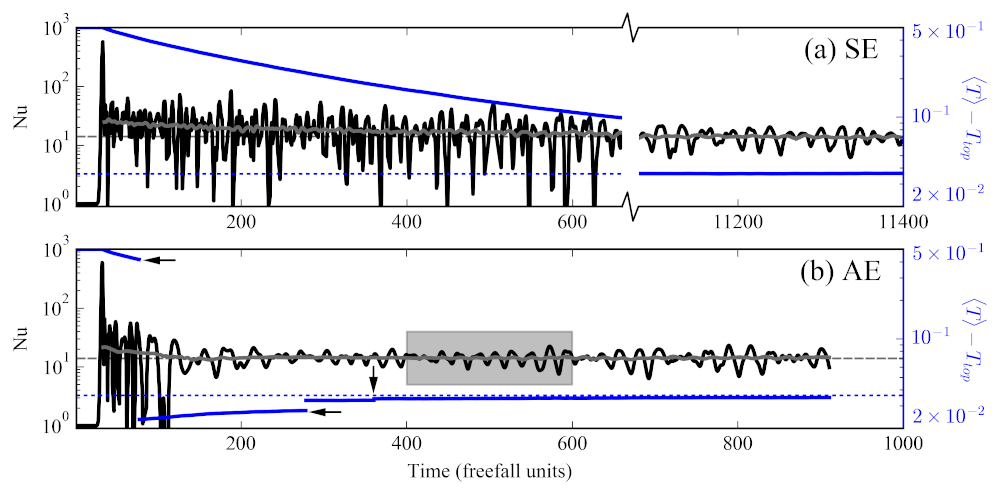
\includegraphics[width=0.48\textwidth]{./figs/nu_v_time.png}
	\vspace{-16pt}
	\end{center}
    \caption{
	\citep[Fig.~2 of][]{anders&all2018} The time evolution of convective transport (black line) and thermal energy (blue line) for a simulation which uses standard timestepping (top) and one which uses our accelerated evolution method (bottom).
	Standard timestepping converges over thousands of convective timescales, but our accelerated evolution method (which occurs at the times marked by arrows) rapidly and accurately achieves the same converged state.
	\label{fig:ae_plot} }
	\vspace{-11pt}
\end{wrapfigure}
Modern simulations of stellar convection generally include a transient phase during which the thermodynamic structure of the domain is relaxing into an equilibrium state.
As simulations are pushed into highly-turbulent, more astrophysically-interesting regimes, this relaxation timescale becomes very long compared to the overturn timescale of convective dynamics.
In state-of-the-art simulations, before meaningful measurements can be taken, this timescale separation creates a long period of rundown which is physically uninteresting and very computationally expensive to timestep through.
In \citet{anders&all2018}, we found a mechanism for fast-forwarding through this equilibration time in a very simple convective system.
We verified that our fast-forwarding procedure produced the same results as standard timestepping techniques to within 1\%.
This accuracy was achieved using an order of magnitude fewer cpu-hours than traditional techniques.
A comparison of an accelerated run and traditional run is shown in Fig.~\ref{fig:ae_plot}.

\paragraph{Entropy Rain: Thermals in Stratified Domains}
\begin{wrapfigure}{l}{0.46\textwidth}
	\begin{center}
	\vspace{-42pt}
    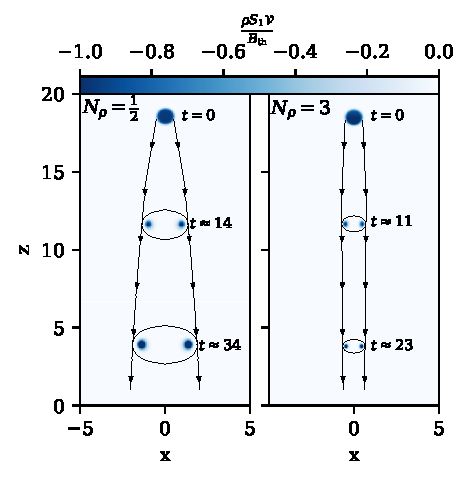
\includegraphics[width=0.45\textwidth]{./figs/evolution_colormeshes.pdf}
	\vspace{-16pt}
	\end{center}
    \caption{
	\citep[Fig.~2 of][]{andersLB2019} Shown is the evolution of the entropy signature in vertical slices through thermals in weakly stratified (left) and highly stratified (right) atmospheres.
	In the presence of weak stratification, these downflows grow with depth; in the presence of strong stratification, they are compressed and they accelerate as they propagate downwards.
	\label{fig:thermals} }
	\vspace{-22pt}
\end{wrapfigure}

Stratified convection, like that in the envelopes of solar-type stars, exhibits asymmetrical flows: upwellings are slow, weak, and wide while downflows are intense, fast, and narrow.
The ``entropy rain'' hypothesis posits that downflows may be so powerful in stellar envelope convection that they alone transport the stellar luminosity, and upflows exist only to conserve mass while transporting negligible energy.
It is possible these downflows turbulently break up into distinct pieces as they fall and these individual downflow pieces can be modeled as ``thermals.''
Thermals are regions of cold fluid which accelerate due to buoyancy forces and shape themselves into vortex rings; thermal evolution is visualized in Fig. \ref{fig:thermals}.

In \citet{andersLB2019}, we studied how an atmospheric density stratification affects the size of thermals as they propagate.
We found that thermals compress less than a simple estimate based on the stratification alone would anticipate \citep{brandenburg2016}.
We further estimated to our surprise that thermal-like downflows could very easily carry the Sun's luminosity through much of the solar convection zone, in agreement with the entropy rain hypothesis.


\vspace{-44pt}
\section*{\textbf{Current \& Ongoing Research}}
As I finish my PhD, I am extending my past research to three small collaborative projects.

\vspace{-4pt}
\paragraph{Individual Downflows Impinging on Stable Layers}
Alongside Prof.~Daniel Lecoanet (Northwestern / Princeton) and Dr.~Lydia Korre (Univ.~Colorado), I am extending my Entropy Rain study to include interactions with the stable layer that lies beneath a solar-like convection zone.
We are trying to determine where the buoyant energy signature of highly resolved downflows is deposited when these flows encounter a stable layer.
In stars, cold downflow material deposited at the base of the convection zone could strongly stabilize that region and suppress flows (such as giant cells) from being driven there \citep{cossette&rast2016}.

\vspace{-4pt}
\paragraph{Thermal Relaxation and Dynamical Regime Changes}
During my PhD, I learned how to set the degree of rotational constraint in a rotating convection simulation \citep{anders&all2019} and I learned how to fast-forward through thermal relaxation \citep{anders&all2018}.
I am collaborating with Prof.~Geoff Vasil (Univ.~Sydney) to study the effects of thermal relaxation on convective simulations when rotation is included.
We have found that at highly turbulent, astrophysically-interesting parameters, the degree of rotational constraint felt by convective flows can change by an order of magnitude between a transient and fully relaxed solution.
As in Fig.~\ref{fig:rossby_plot}, changing the degree of rotational constraint greatly alters the convective flow structures, and we are trying to determine if this massive change of rotational influence leaves hysteretic effects which may pollute simulation results.

\vspace{-4pt}
\paragraph{Predicting the Rossby Number in Global Simulations}
The simulations I conducted in \citet{anders&all2019} showed that the degree of rotational constraint could be set \emph{a priori} in \emph{Cartesian} simulations of rotating convection.
Dr.~Nick Featherstone (Univ.~Colorado) and I are currently investigating whether or not this can be achieved in convective simulations in spherical geometries.
Past work by \citet{featherstone&hindman2016} shows that the degree of rotational constraint felt by convective flows in a global simulation can vastly change the evolved flow structures, and so verifying our mechanism in global simulations is crucial.


\bibliographystyle{../yahapj}
\bibliography{../biblio}
\end{document}
